\chapter{INTRODUCTION}
\label{chap-one}

Persistent memory faults represent one of the most serious long-term risks to embedded system reliability. When non-volatile storage such as flash, EEPROM, or ROM becomes corrupted, the stored program image itself is damaged. Unlike disturbances in volatile components, persistent faults survive power cycles and reboots. As a result, the system repeatedly executes corrupted instructions or loads incorrect configuration data on every startup. Without safeguards, the device can become unresponsive, behave unpredictably, or fail to boot entirely. In many embedded deployments, even a single corrupted byte can disable critical initialization logic, break peripheral configuration, or block firmware updates---potentially requiring external re-flashing or hardware replacement.

Persistent faults are especially dangerous during system initialization. Early boot code executes before watchdogs, operating systems, or repair logic are active, and before any trusted memory state has been established. At this point, every instruction fetch and data load relies directly on raw, potentially corrupted persistent memory. If corruption prevents the boot sequence from reaching a stable operating state, the processor may stall, repeatedly reset, or fail to configure essential subsystems. Because no fault-tolerance mechanism is yet available, the system has no way to detect corruption or select a clean execution path. A single fault at this stage can permanently trap the device in an unrecoverable condition until external intervention occurs.

Early boot execution is dominated by instructions rather than mutable data. Initialization routines follow a strict, deterministic sequence: configuring clocks and memory, initializing registers, verifying system state, and preparing the software environment. These steps consist almost entirely of instruction fetches and control transfers, with minimal dynamic data processing. Since the boot path uses little writable state and relies on static program storage, the correctness of instruction memory becomes the primary determinant of whether the system reaches operational mode. A single corrupted opcode, branch target, or startup constant can halt progress long before any recovery logic can be invoked.

The processor's memory architecture shapes what recovery mechanisms are even possible in the presence of persistent faults. In a Harvard architecture, instructions and data occupy physically separate memory spaces accessed through distinct pathways. Executable code cannot be modified through normal load/store operations, meaning firmware cannot repair or regenerate corrupted instruction memory at runtime. Recovery typically requires an external programmer or supervisory controller. In a Von Neumann architecture, instructions and data share a unified address space. Here, firmware can potentially construct or repair executable code dynamically, enabling self-stabilization or redirection---but only after the system reaches a sufficiently functional state to run such logic. Until that point, memory corruption threatens the boot path in exactly the same way. Persistent faults pose equal risk under both models. The distinction is structural: Harvard machines cannot rewrite instruction memory at runtime, forcing recovery to come from external intervention; Von Neumann machines may enable software-based repair or redirection---but only if execution survives long enough to activate those mechanisms.

Most software reliability mechanisms are designed to protect against transient faults that affect registers, pipelines, or RAM during execution. Compilers insert redundancy around loads, stores, branches, and function calls to detect unexpected state changes and correct them through re-execution or value checks. However, these protections activate only after instructions have been successfully fetched and executed. If the instruction stream itself is corrupted in flash or ROM, execution follows a deterministic faulty path on every boot. The inserted checks never run because the very instructions that would perform them may be unreachable or corrupted. Thus, traditional compiler-assisted hardening does not protect against persistent instruction faults. It assumes a correct instruction stream and attempts to repair data state after faults arise---not to validate code before it executes. When faults exist in persistent program storage, failure can occur before software recovery logic is ever reached.


\section{Static Memory and Instruction Reliability}
\label{sec:static-memory-instr-reliability}

Whether running on a microcontroller or a general-purpose computer, most of a program’s bytes are stored in fixed sections like \texttt{.text}, \texttt{.rodata}, and \texttt{.data}. These bytes originate in persistent memory and must be read correctly for the program to execute as intended. Because they form the backbone of execution and persist across resets, any corruption in these regions becomes a permanent part of program behavior, making static code and data integrity the primary driver of long-term reliability.

Figure~\ref{fig:section-breakdown-embedded} shows this breakdown for a set of embedded benchmark programs. These workloads, drawn from real-time and control-oriented software, are overwhelmingly dominated by static content. The \texttt{.text} region---executable instructions---makes up the largest share, followed by \texttt{.rodata}, with \texttt{.data} representing only a small fraction. Because the instruction stream defines control flow and executes continuously, even a single corrupted byte in \texttt{.text} can alter program behavior, break control logic, or disable essential routines. This concentration of static code underscores why protecting persistent instruction memory is critical for system reliability.

The \texttt{.rodata} region contains fixed constants that the program depends on---lookup tables, configuration values, cryptographic material, and calibration coefficients. While these bytes are not executed as instructions, they define the logic and numerical behavior of the software. A single corrupted constant can silently change outputs, break protocol behavior, or push control algorithms into unstable regimes. Because \texttt{.rodata} persists across reboots and is never rewritten by normal execution, such faults are repeatable and difficult to diagnose: the system consistently behaves incorrectly without crashing, masking the failure as a logic or calibration issue.

The \texttt{.data} section contrasts with \texttt{.rodata} in mutability, not origin. Its initial values are also stored in non-volatile memory and copied into RAM at startup. Before this transfer occurs, \texttt{.data} is just as vulnerable as \texttt{.rodata}: a corrupted value in persistent storage is loaded directly into RAM and drives deterministic incorrect behavior. Only after initialization does \texttt{.data} become writable and able to absorb transient faults. Until that first copy completes, \texttt{.data} faults behave like static corruption rather than dynamic state errors, reinforcing the importance of protecting the stored program image before execution begins.

% --- Figure 1: Embedded benchmarks ---
\begin{figure}[t]
  \centering
  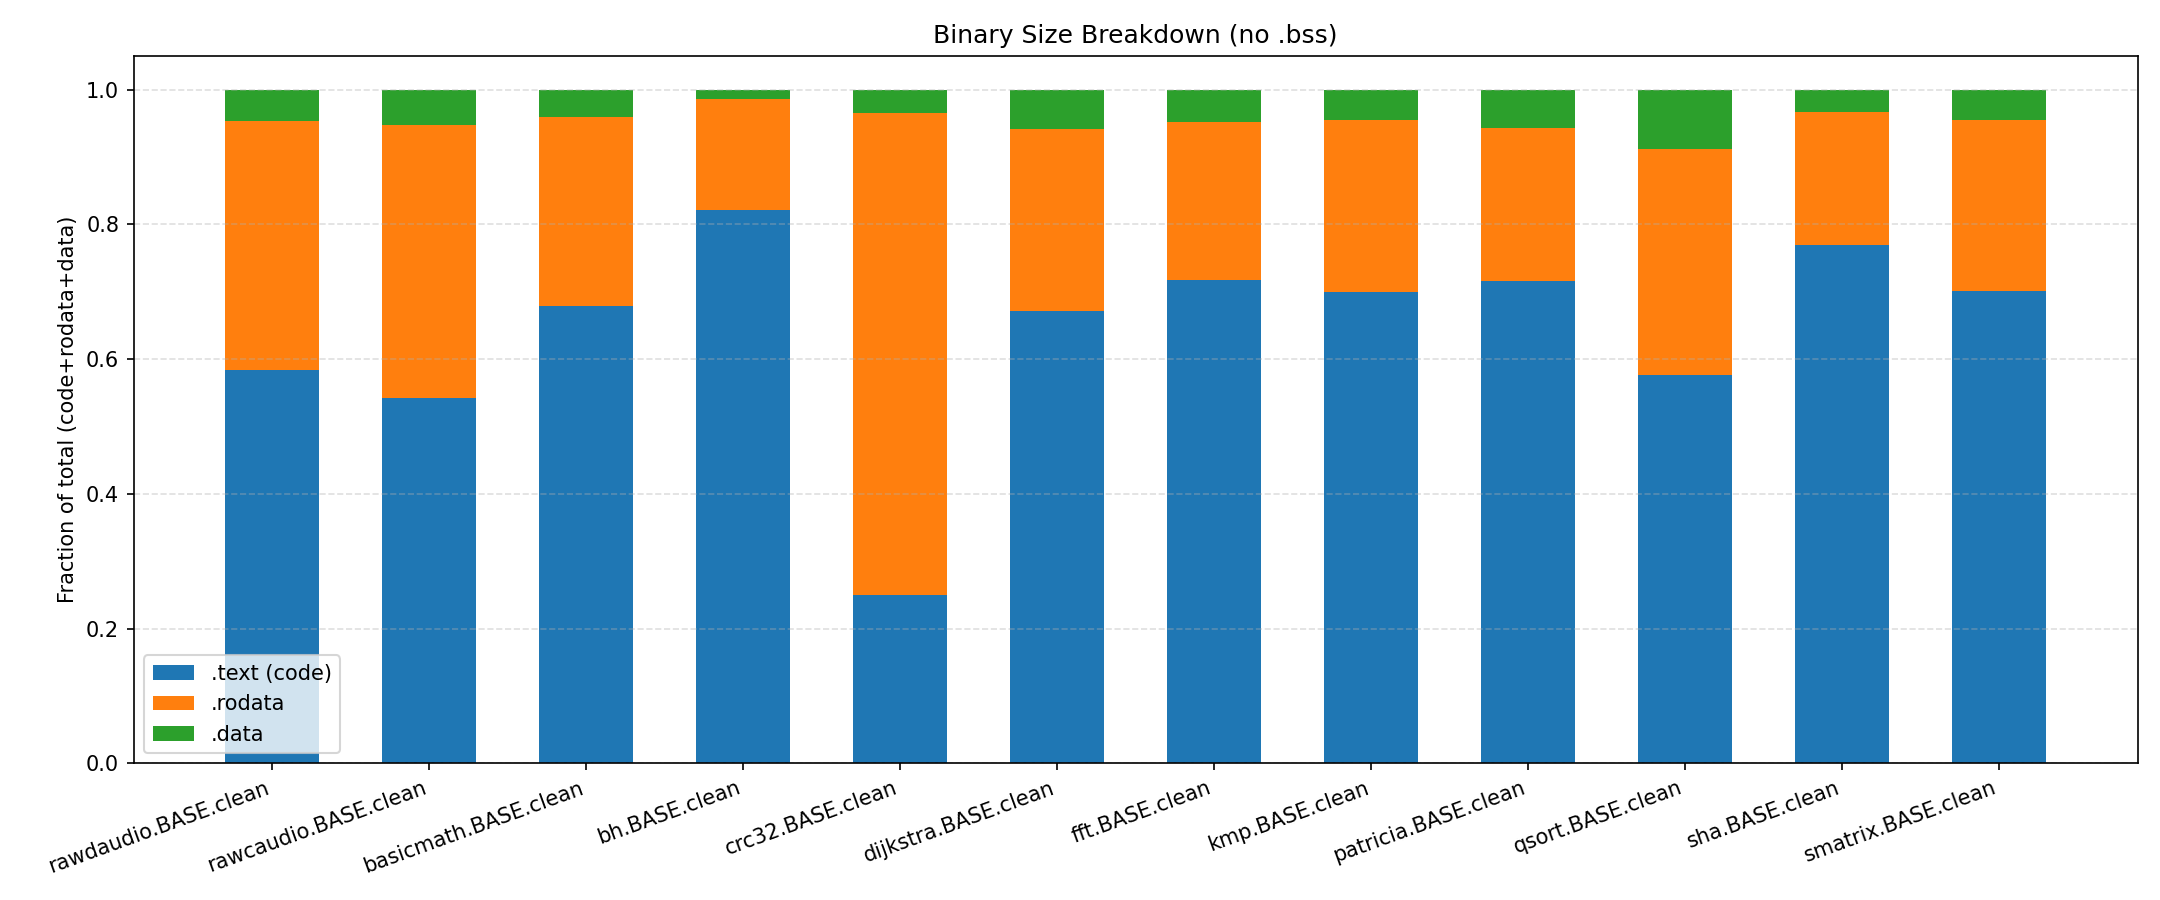
\includegraphics[width=0.86\linewidth]{Chapter-1/figs/embedded-bin.png}
  \caption{Representative embedded benchmarks compiled for ARM targets. The \texttt{.text} section dominates, followed by smaller fractions of \texttt{.rodata} and \texttt{.data}.}
  \label{fig:section-breakdown-embedded}
\end{figure}

% --- Figure 2: General-purpose binaries (Apple M2) ---
\begin{figure}[t]
  \centering
  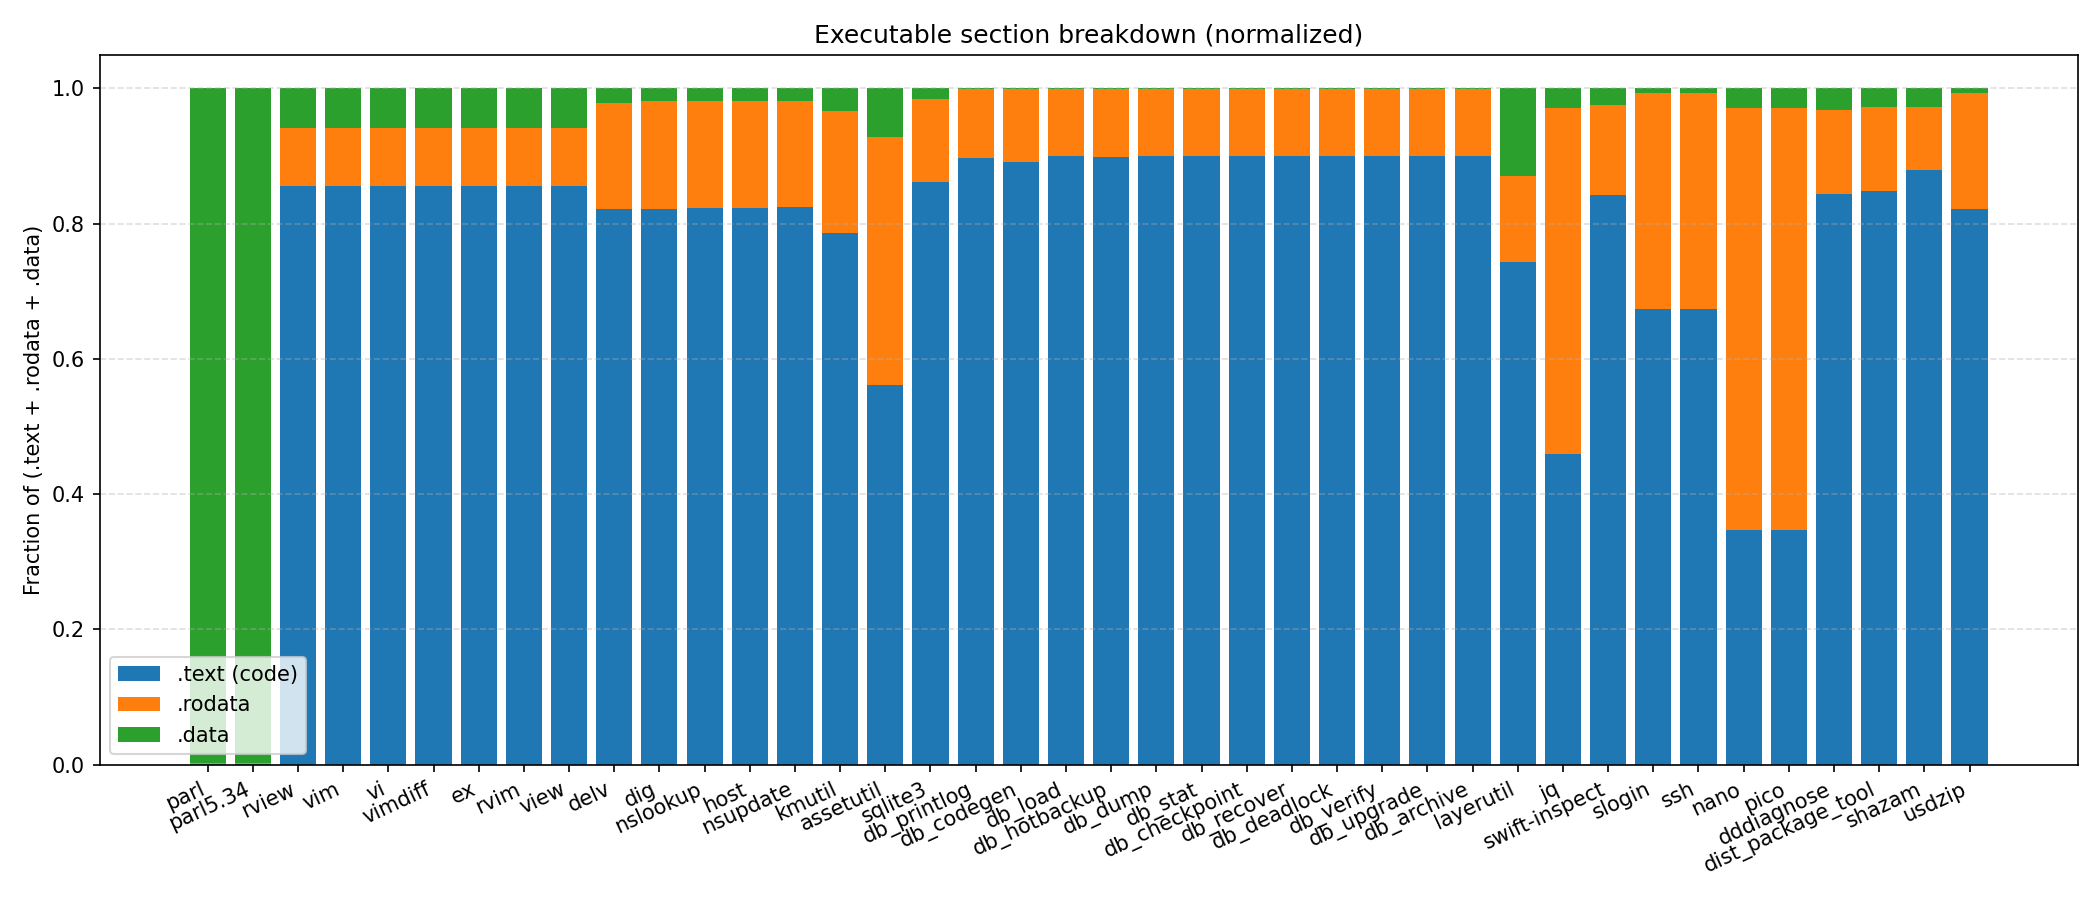
\includegraphics[width=0.86\linewidth]{Chapter-1/figs/apple-bin.png}
  \caption{User-space binaries compiled for an Apple M2 processor show the same bias toward static code and read-only data across diverse applications.}
  \label{fig:section-breakdown-m2}
\end{figure}

A similar pattern appears in general-purpose software (Figure~\ref{fig:section-breakdown-m2}). Across applications ranging from utilities and interpreters to media tools and network services, the \texttt{.text} section remains the dominant component of the binary, followed by \texttt{.rodata}. Writable \texttt{.data} is comparatively small. This consistency across domains shows that modern binaries are overwhelmingly composed of code and statically initialized data rather than transient runtime state. Because these sections originate in persistent storage, faults in them do not dissipate---they reappear identically on every boot and every fetch. In contrast, transient errors in volatile memory may be overwritten or corrected by normal execution. Thus, protecting and validating \texttt{.text}, \texttt{.rodata}, and initial \texttt{.data} before execution begins is essential to ensuring long-term system reliability.

Modern reliability mechanisms such as error-correcting codes, parity protection, and data replication can successfully guard \texttt{.data} and \texttt{.rodata}, since these regions can be validated and repaired using redundant copies or mathematical consistency checks. However, the same techniques are far less effective for the \texttt{.text} section. The instruction stream must remain executable, ordered, and semantically intact—properties that are easily broken by even small changes in opcode bytes. Moreover, instruction redundancy itself increases exposure: methods such as triple modular redundancy (TMR) and SWIFT-R multiply the number of instructions that must be fetched and executed. TMR expands the instruction footprint by roughly three times, while SWIFT-R approaches a fourfold increase. Thus, even though these schemes improve fault coverage in data paths, they enlarge the surface of persistent vulnerability in instruction memory, further emphasizing the need for techniques that validate and protect \emph{code regions directly} rather than relying solely on post-execution recovery.



\section{Memory Hardening: Data and Instruction Paths}

Memory hardening techniques improve the likelihood of correct program execution in the presence of faults that affect code or data. These approaches can be divided into two domains: \textbf{data-path hardening}, which strengthens reliability within the dynamic state of a running program, and \textbf{instruction-path hardening}, which reduces the probability that corruption in persistent memory disrupts control flow. While both address different fault conditions, they operate in a complementary manner to sustain coherent execution.

\subsection{Data-Path Hardening}

Data-path hardening improves reliability as data moves through the system during computation. Compilers introduce validation checks around memory operations—verifying values at load, confirming address bounds, and checking results before store—to identify disturbances while data is in motion. Redundant encodings, shadow memory, and arithmetic schemes such as AN codes further suppress error propagation by maintaining predictable relationships among stored values. These mechanisms increase the likelihood that transient disturbances are absorbed or corrected before they affect program state.

Additional measures strengthen the transformation stage of computation. Compilers may recompute selected expressions, maintain arithmetic invariants, or mirror dependence chains so that register values are cross-checked before commit. Each added check improves the consistency of intermediate state and raises confidence that computation proceeds as intended. These techniques reinforce runtime stability but depend on correct instruction delivery; when the instruction stream itself is corrupted, validation logic may not execute as designed.

Because these protections activate only after instructions are fetched and decoded, they cannot isolate faults that prevent code from executing normally. Furthermore, redundancy introduces modest increases in code size, fetch bandwidth, and register pressure, slightly expanding the instruction memory exposed to long-term corruption. Data-path hardening therefore improves runtime robustness while emphasizing probabilistic containment of transient effects.

\subsection{Instruction-Path Hardening}

Instruction-path hardening operates before execution to strengthen the reliability of code fetched into the processor. It targets the \texttt{.text} section of memory—typically flash or other non-volatile storage—where faults persist across resets and reappear on every fetch. Even small disturbances in this region can redirect control flow, disable protection logic, or block initialization. Instruction-path hardening improves the likelihood that execution progresses through coherent, structurally consistent code despite these faults.

Two broad strategies contribute to this improvement: \textbf{repair} and \textbf{redirection}.  
\textbf{Repair} treats code as a regenerable entity produced through algorithmic synthesis. It generates new data according to defined transformation rules, and when this data occupies instruction memory, it is interpreted as executable code. Instruction formation emerges as a natural consequence of the repair process. The method operates in a feed-forward manner, constructing new code regions that extend execution beyond corrupted states through algorithmic continuity rather than direct restoration.

\textbf{Redirection} improves reliability through replication. The program contains multiple prevalidated copies of key code regions and selects among them at runtime. When corruption is detected, control transfers to a clean replica, maintaining execution without dependence on a single static region.  

Redirection can be organized at multiple structural levels. At the coarsest scale, \textbf{image-based redirection} replaces the entire binary as a single executable region. \textbf{Section-based redirection} partitions the program along segment boundaries: the \texttt{.data} and \texttt{.rodata} sections remain fixed, while the \texttt{.text} section—containing executable instructions—can be revalidated or replaced independently.  
\textbf{Function-level redirection} aligns with natural control-flow boundaries, substituting routines when corruption is detected at entry points. \textbf{Basic-block redirection} extends this precision, verifying smaller control-flow segments and bypassing localized corruption to maintain program continuity. At the finest scale, \textbf{instruction-level redirection} validates or substitutes individual opcodes before execution. At this level, the process resembles controlled self-modifying code: short, verified instruction sequences are dynamically reconstructed and executed as the program advances. The original code serves as an input template for generating a syntactically coherent instruction stream. Although this approach increases metadata and control complexity, it significantly raises the likelihood of sustained execution under fault conditions.

Together, repair and redirection establish a hierarchy of probabilistic defense. Coarse-grained methods are simple and broad, while fine-grained techniques capture localized corruption with greater precision. Each level contributes to maintaining coherent execution paths and extending operational continuity in imperfect memory environments.

\subsection{Integration and Limitations}

Both forms of hardening act on different temporal and structural dimensions of execution. \textbf{Data-path mechanisms} strengthen reliability within the dynamic state of a running program, detecting and containing transient faults that arise during runtime computation. \textbf{Instruction-path mechanisms} operate before execution, improving the consistency of code fetched from static memory. The two domains reinforce each other: instruction hardening stabilizes code delivery, while data hardening preserves state integrity once execution begins.

Redundancy enhances reliability but also expands the volume of instruction memory that must remain correct. Additional checks, replicated regions, and control-flow guards multiply the number of instructions required to maintain consistency. Techniques such as triple modular redundancy (TMR) or SWIFT-R expand the instruction footprint by several factors—improving resilience to transient errors but proportionally enlarging the memory exposed to persistent faults. Effective design balances these effects, increasing reliability through selective replication rather than uniform duplication.

In summary, memory hardening raises the probability that computation proceeds coherently even under fault conditions. It biases execution toward successful outcomes through redundancy, regeneration, and control-flow redirection. Data-path and instruction-path mechanisms together define a continuum of resilience—one that enables forward progress in systems that must operate under imperfect, noisy, or degraded hardware environments.


\subsection{Hardware Constraints}

Hardware characteristics strongly influence the feasibility and effectiveness of repair and redirection. These mechanisms depend on the ability to modify or replace code regions, and their practicality is shaped by the memory architecture and performance capabilities of the target device.

\textbf{Redundancy cost.}  
Redundancy consumes a portion of the available static memory storage and contributes directly to implementation overhead. Each replica, checksum, or repair table occupies additional non-volatile space, reducing capacity available for primary code or data. On memory-constrained platforms such as microcontrollers and deeply embedded processors, this limits the granularity and extent of replication. The trade-off is multidimensional: greater redundancy increases coverage but requires more storage, while more sophisticated repair or encoding algorithms can reduce redundancy at the expense of higher algorithmic complexity and reduced performance. Designers must balance these factors—storage overhead, computational cost, and execution speed—to achieve meaningful improvements in reliability without exceeding system constraints.

\textbf{Write access.}  
Repair requires writable storage to regenerate or update code regions. In many embedded systems, memory is divided by access type: some areas are fully writable, others are one-time programmable (OTP), and others are permanently read-only. Flash memory often supports region-level protection, allowing selected segments to be locked behind read-only boundaries once programming is complete. Edge devices may further restrict writes from the main processor, allowing modification only through external programmers or management controllers. These constraints determine where repair can take place and how redirection metadata can be safely stored without violating device security or memory access policy.

\textbf{Flash memory limitations.}  
Flash memory endurance directly limits the frequency of repair and update operations. Each Program/Erase (P/E) cycle physically degrades storage cells, and repeated rewriting accelerates wear, leading to retention loss and eventual data failure. As degradation accumulates, affected flash sectors may become uncorrectable, exceeding the capability of onboard error correction codes (ECC) and rendering the section permanently unreliable. Relocating or rewriting instruction regions across flash sectors further increases the rate at which these cells fail and shortens overall device lifetime. Consequently, repair operations must minimize the number of write and erase events, favor localized correction, and confine updates to small, managed regions.

\textbf{RAM capacity and volatility.}  
RAM offers a writable and low-latency medium for storing repaired or reconstructed code, but it is physically smaller and volatile. The limited capacity restricts how much code can be regenerated or redirected at once, especially on devices with only a few hundred kilobytes of memory. Volatility also means that repaired code vanishes on power loss, requiring regeneration at each startup. This makes RAM-based repair practical for transient correction or runtime reconstruction but unsuitable for persistent code recovery without complementary non-volatile storage.

\textbf{Performance.}  
The performance impact of hardening arises from the additional computation and control steps introduced by repair and redirection. Repair algorithms increase instruction latency by generating or reconstructing data during execution, consuming cycles and memory bandwidth that would otherwise serve program logic. Simpler repair methods minimize this delay but offer limited tolerance to complex corruption, while more advanced regeneration schemes incur longer processing times and temporary buffer usage.  
Redirection alters control flow by inserting validation and target-selection logic, introducing extra jumps and synchronization points that reduce pipeline efficiency. Fine-grained redirection, especially at the basic-block or instruction level, amplifies instruction fetch and branch overhead. Both repair and redirection can disrupt caching and locality, as reconstructed or alternate code regions may occupy different memory locations than the originals. These effects collectively determine how much resilience can be achieved before performance degradation outweighs reliability gains.


\section{Related Work}

Research on fault tolerance has produced extensive techniques for detecting and recovering from transient faults in the data path, yet far less attention has been given to faults that reside in persistent instruction memory. Most existing approaches focus on maintaining correct execution after faults occur rather than preventing faulty code from entering execution in the first place. The following works summarize the main directions in software-based reliability and highlight the gap in fine-grained protection for static instruction regions.

Most reliability work targets the data path. Many systems rely on detection followed by reset or replay, which is effective for transient faults that clear when the state is refreshed. General-purpose operating systems can impose time limits or kill runaway processes to recover forward progress. Edge devices often use a watchdog timer for the same purpose. These responses restore execution but do not address corruption that persists in code storage.

Irregular control is commonly handled with control flow checking. Software Implemented Fault Tolerance systems combine control flow checking with replication of dependence chains so that computations can be compared during execution. These approaches detect many dynamic faults and can force recovery when a mismatch is observed. They still execute checks after instructions have been fetched and decoded, so they depend on an intact instruction stream and do not directly protect code bytes in static memory.

For errors in static instruction memory, there is little direct software support. Indirect measures can raise baseline reliability. A dual-image bootloader maintains two program images and selects one at startup based on the validation of integrity. When images are identical, this creates replication at the image level, and vendors describe such A/B update schemes in application notes and design guides. Selection and validation can occur in firmware or in hardware at boot. However, these mechanisms act at coarse granularity and do not validate, repair, or redirect at the level of individual functions or blocks during normal execution.

In summary, prior work focuses on data protection, on recovery by reset or replay, and on run-time checks of control behavior. Direct hardening of instruction memory remains limited. The gap is a lack of methods that perform pre-execution validation of code and then repair or redirect at fine granularity so that control follows a clean path through validated regions.

\section{Purpose of this Thesis}

This thesis examines the reliability of instruction memory in the presence of faults and explores software-based strategies to improve system resilience. The work centers on two complementary approaches: \textbf{code repair}, which reconstructs executable content from damaged regions, and \textbf{code replication}, which provides alternate copies of code that can be selected when corruption is detected. Both approaches are coordinated through \textbf{pre-execution validation}, increasing the overall reliability of the system by ensuring that execution proceeds through trustworthy instruction paths.

Together, these techniques represent a shift from protecting transient runtime state to reinforcing the integrity of static program storage. By addressing faults that originate in instruction memory, this work extends reliability coverage beyond the data path and provides a foundation for continued operation even when parts of the program image are compromised.

The thesis evaluates the impact of these techniques across multiple dimensions, including their effects on \textbf{performance}, \textbf{reliability}, \textbf{storage cost}, and \textbf{code overhead}. It further examines the conditions under which each approach is most effective, identifying the trade-offs that arise between protection strength, system resources, and operational constraints.